\documentclass{article}
\usepackage[backend=biber,natbib=true,style=authoryear,maxbibnames=10]{biblatex}
\addbibresource{/home/nqbh/reference/bib.bib}
\usepackage[utf8]{vietnam}
\usepackage{tocloft}
\renewcommand{\cftsecleader}{\cftdotfill{\cftdotsep}}
\usepackage[colorlinks=true,linkcolor=blue,urlcolor=red,citecolor=magenta]{hyperref}
\usepackage{amsmath,amssymb,amsthm,float,graphicx,mathtools,tikz}
\usetikzlibrary{angles,calc,intersections,matrix,patterns,quotes,shadings}
\allowdisplaybreaks
\newtheorem{assumption}{Assumption}
\newtheorem{baitoan}{Bài toán}
\newtheorem{cauhoi}{Câu hỏi}
\newtheorem{conjecture}{Conjecture}
\newtheorem{corollary}{Corollary}
\newtheorem{dangtoan}{Dạng toán}
\newtheorem{definition}{Definition}
\newtheorem{dinhly}{Định lý}
\newtheorem{dinhnghia}{Định nghĩa}
\newtheorem{example}{Example}
\newtheorem{ghichu}{Ghi chú}
\newtheorem{hequa}{Hệ quả}
\newtheorem{hypothesis}{Hypothesis}
\newtheorem{lemma}{Lemma}
\newtheorem{luuy}{Lưu ý}
\newtheorem{nhanxet}{Nhận xét}
\newtheorem{notation}{Notation}
\newtheorem{note}{Note}
\newtheorem{principle}{Principle}
\newtheorem{problem}{Problem}
\newtheorem{proposition}{Proposition}
\newtheorem{question}{Question}
\newtheorem{remark}{Remark}
\newtheorem{theorem}{Theorem}
\newtheorem{vidu}{Ví dụ}
\usepackage[left=1cm,right=1cm,top=5mm,bottom=5mm,footskip=4mm]{geometry}
\def\labelitemii{$\circ$}
\DeclareRobustCommand{\divby}{%
	\mathrel{\vbox{\baselineskip.65ex\lineskiplimit0pt\hbox{.}\hbox{.}\hbox{.}}}%
}

\title{TikZ}
\author{Nguyễn Quản Bá Hồng\footnote{Independent Researcher, Ben Tre City, Vietnam\\e-mail: \texttt{nguyenquanbahong@gmail.com}; website: \url{https://nqbh.github.io}.}}
\date{\today}

\begin{document}
\maketitle
\begin{abstract}
	A personal practice of drawing figures in \LaTeX\ by using TikZ package.
\end{abstract}
\tableofcontents

%------------------------------------------------------------------------------%

\section{Coordinate System -- Hệ Trục Tọa Độ}
See \cite{Quy2022}.

\begin{tikzpicture}[>=stealth,scale=.75]
	\draw[->](-3,0)--(3,0) node[above]{$x$};
	\draw[->](0,-3)--(0,3) node[left]{$y$};
	\draw[dashed](0,1)--(2,1)--(2,0);
	\draw(2,1) circle(0.05) node[above right]{$A$};
	\path(0,0) node [below left]{$O$};
\end{tikzpicture}
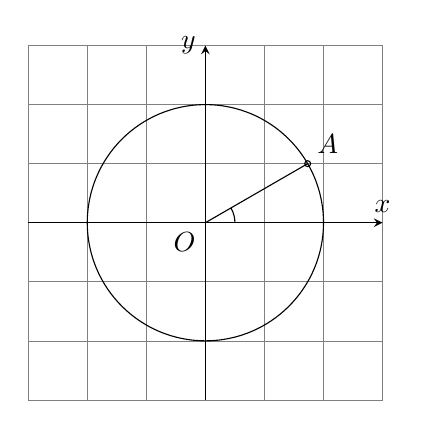
\begin{tikzpicture}[>=stealth,scale=.75]
	\draw[step=1,gray,very thin](-3,-3) grid (3,3);
	\draw[->](180:3)--(0:3) node[above]{$x$};
	\draw[->](-90:3)--(90:3) node[left]{$y$};
	\draw(0,0) circle(2);
	\draw(0,0)--(30:2) (0:.5) arc(0:30:.5);
	\draw(30:2) circle(0.05) node[above right]{$A$};
	\path(0:0) node[below left]{$O$};
\end{tikzpicture}

\begin{tikzpicture}
	\draw[step=1,gray,very thin](-2,-1) grid (3,2);
\end{tikzpicture}

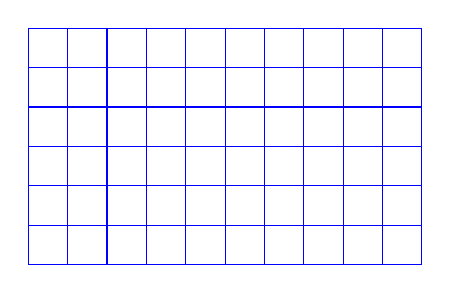
\begin{tikzpicture}
	\draw[step=.5,blue,thin](-2,-1) grid (3,2);
\end{tikzpicture}
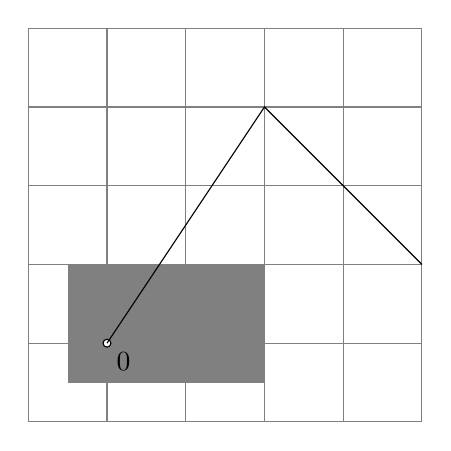
\begin{tikzpicture}
	\draw[step=1,gray,thin](-1,-1) grid (4,4);
	\fill[gray](-.5,-.5) rectangle (2,1);
	\draw[fill=white] (0:0) circle (.05);
	\draw(0:0)--(2,3)--(4,1);
	\path(0:0) node[below right]{$0$};
\end{tikzpicture}
\begin{tikzpicture}[declare function={c=sqrt(3);}]
	\coordinate[label=above:A](A) at (1,2);
	\coordinate (A) at (30:2);
	\path
	(1,2) coordinate[label=above:A] (A)
	(2,5) coordinate[label=right:B] (B)
	(4,2) coordinate[label=left:C] (C)
	%\coordinate (H) at ($(A)+(B)$)
	%\coordinate[label=above:D] (D) at ($(A)!.5!(B)$)
	%\coordinate (E) at ($(A)!1!30:(B)$)
	%\coordinate (F) at ($(A)!.5!30:(B)$)
	%\coordinate (G) at (intersection of A--B and C--D)
	;
	\def\a{3}
	\pgfmathsetmacro\b{2*sqrt(2)}
	\draw (0:0) circle (\a);
	\draw (0:0) circle (c);
\end{tikzpicture}

\section{Triangle -- Tam Giác}

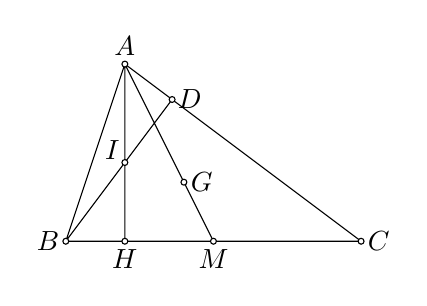
\begin{tikzpicture}[scale=.75]
	\path
	(1,3) coordinate (A)
	(0,0) coordinate (B)
	(5,0) coordinate (C)
	($(B)!(A)!(C)$) coordinate (H)
	($(A)!(B)!(C)$) coordinate (D)
	(intersection of A--H and B--D) coordinate (I)
	($(B)!.5!(C)$) coordinate (M) %barycentric cs:B=1.C=1
	(barycentric cs:A=1,B=1,C=1) coordinate (G);
	\draw (A)--(B)--(C)--cycle (A)--(H) (A)--(M) (B)--(D)
	;
	\foreach \x/\g in {A/90,B/180,C/0,H/-90,D/0,I/135,M/-90,G/0} \draw[fill=white] (\x) circle (.05) + (\g:.3) node{$\x$};
\end{tikzpicture}
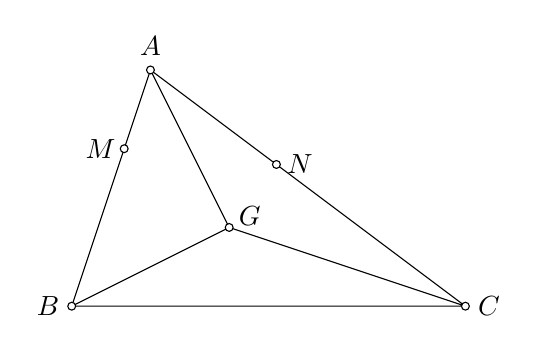
\begin{tikzpicture}
	\path
	(1,3) coordinate (A)
	(0,0) coordinate (B)
	(5,0) coordinate (C)
	(barycentric cs:A=1,B=1,C=1) coordinate (G)
	(barycentric cs:A=2,B=1) coordinate (M)
	(barycentric cs:A=3,C=2) coordinate (N)
	;
	\draw (A)--(B)--(C)--cycle (A)--(G)--(B) (G)--(C);
	\foreach \x/\g in {A/90,B/180,C/0,M/180,N/0,G/30} \draw[fill=white] (\x) circle (.05) + (\g:.3) node{$\x$};
\end{tikzpicture}
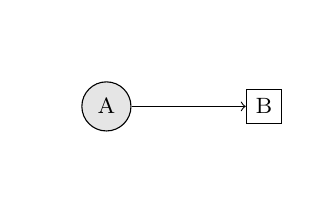
\begin{tikzpicture}[font=\footnotesize]
	\clip(-1,1) rectangle (2.5,-1);
	\node[circle,fill=gray!20,draw] (A) at (0,0){A};
	\node[rectangle,draw] (B) at (2,0){B};
	\draw[->] (A)--(B);
\end{tikzpicture}
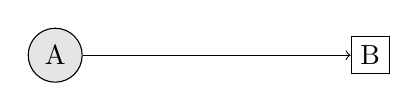
\begin{tikzpicture}
	\path
	(0,0) node[circle,fill=gray!20,draw] (A) {A}
	(4,0) node[rectangle,draw] (B) {B}
	;
	\draw[->] (A)--(B);
\end{tikzpicture}
\begin{tikzpicture}
	%\path (0,0) node (tree) {\includegraphics[scale=.25]{a}};
	%\draw (tree.north) -- (tree.south) --++ (4,0) -- cycle;
\end{tikzpicture}
\begin{tikzpicture}
	\draw(3,-1) circle (1pt);
	\draw(60:2) circle (1pt);
\end{tikzpicture}

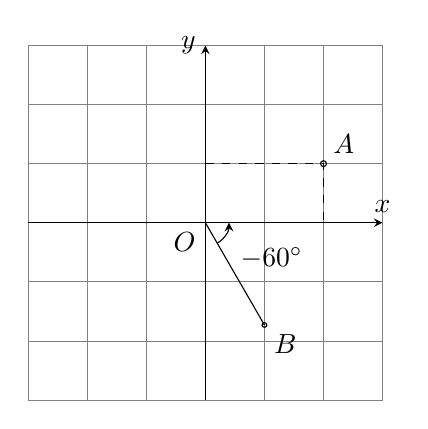
\begin{tikzpicture}[>=stealth,scale=.75]
	\draw[step=1,gray,very thin](-3,-3) grid (3,3);
	\draw[->](-3,0)--(3,0);
	\draw[->](0,-3)--(0,3);
	\draw[dashed](0,1)--(2,1)--(2,0);
	\draw(2,1) circle(.05);
	\draw(3,0) node[above]{$x$} (0,3) node[left]{$y$} (0,0) node[below left]{$O$};
	\draw(-60:2) circle(0.04);
	\draw(-60:2) -- (0,0);
	\draw(2,1) node[above right]{$A$} (-60:2) node[below right]{$B$};
	\draw[->](-60:4mm) arc(-60:0:4mm);
	\path(-30:5mm) node[below right]{$-60^\circ$};
\end{tikzpicture}
\begin{tikzpicture}
	\path
	(0:0) coordinate (A)
	(2,1) coordinate (B)
	(3,2) coordinate (C)
	(4,1) coordinate (D)
	;
	\draw (A)--(B)--(C)--(D);
	\draw (A)--(B)--++(1,2)--++(1,-1);
	\foreach \x/\g in {A/180,B/120,C/90,D/0} \draw[fill=white] (\x) circle (.05) + (\g:.3) node{$\x$};	
\end{tikzpicture}
\begin{tikzpicture}
	\def\a{2}
	\draw (0:0)--++(0:\a)--++(45:\a)--++(135:\a)--++(180:\a);
\end{tikzpicture}
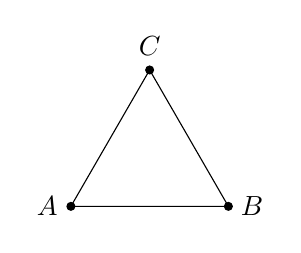
\begin{tikzpicture}
	\draw(0,0) coordinate (A) -- (2,0) coordinate (B) -- ([turn]120:2) coordinate (C)--cycle;
	\foreach \x/\g in {A/180,B/0,C/90} \draw[fill=black] (\x) circle (.05) + (\g:.3) node{$\x$};
\end{tikzpicture}

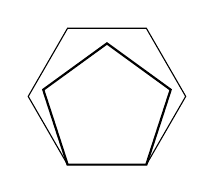
\begin{tikzpicture}
	\def\a{1}
	\draw[thick](0:0) --++ (72:\a) -- ([turn]72:\a) -- ([turn]72:\a) -- ([turn]72:\a) -- cycle;
	\draw(0:0) --++ (60:\a) -- ([turn]60:\a) -- ([turn]60:\a) -- ([turn]60:\a) -- ([turn]60:\a) -- cycle;
\end{tikzpicture}
\begin{tikzpicture}
	\draw(0,0) rectangle (4,2);
\end{tikzpicture}

\section{Curve -- Đường Cong}

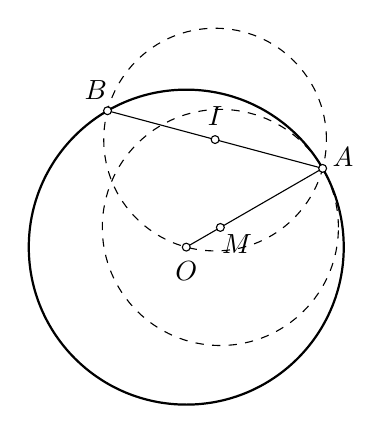
\begin{tikzpicture}
	\def\r{2}
	\path
	(0:0) coordinate (O)
	(30:\r) coordinate (A)
	(120:\r) coordinate (B)
	($(A)!.5!(B)$) coordinate (I)
	($(O)!.25!(A)$) coordinate (M)
	;
	\draw[thick] (O) circle (\r);
	\draw[dashed] let\p1=($(I)-(A)$), \p2=($(M)-(A)$) in (I) circle ({veclen(\x1,\y1)}) (M) circle({veclen(\x2,\y2)});
	\draw(O)--(A)--(B);
	\foreach \x/\g in {O/-90,A/30,B/120,I/90,M/-45} \draw[fill=white] (\x) circle (.05) + (\g:.3) node{$\x$};
\end{tikzpicture}
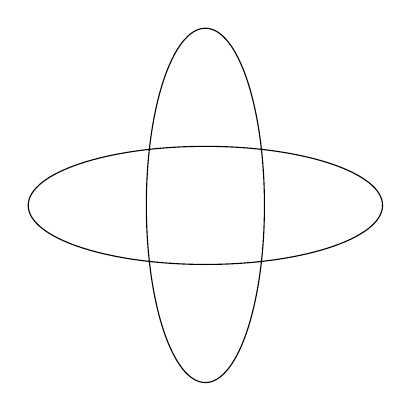
\begin{tikzpicture}[scale=.75]
	\draw(0:0) ellipse ({3} and {1}) (0:0) ellipse ({1} and {3});
\end{tikzpicture}
\begin{tikzpicture}
	\draw(0,0) arc (180:90:2);
	\draw(0,0) arc (180:0:{2} and {1});
\end{tikzpicture}
\begin{tikzpicture}
	\path
	(0,0) coordinate (A)
	(4,3) coordinate (B)
	;
	\draw (A)to[bend left=30] (B);
	\draw[dashed] (A)to[bend right=30] (B);
	\foreach \x/\g in {A/-150,B/60} \draw[fill=white] (\x) circle (.05) + (\g:.3) node{$\x$};
\end{tikzpicture}

\begin{tikzpicture}
	\path (0,0) coordinate (A) (4,3) coordinate (B);
	\draw(A)to[out=90,in=30](B);
	\draw[dashed](A)to[out=0,in=90](B);
	\foreach \x/\g in {A/-150,B/60} \draw[fill=white] (\x) circle (.05) + (\g:.3) node{$\x$};
\end{tikzpicture}
\begin{tikzpicture}
	\path (0,0) coordinate (A) (2,3) coordinate (B);
	\draw(A) parabola (B);
	\draw[dashed](A) parabola[bend at end] (B);
	\foreach \x/\g in {A/-150,B/60} \draw[fill=white] (\x) circle (.05) + (\g:.3) node{$\x$};
\end{tikzpicture}
\begin{tikzpicture}
	\path (0,0) coordinate (A) (3,2) coordinate (B) (4,1) coordinate (C);
	\draw(A) parabola bend (B) (C);
	\foreach \x/\g in {A/-150,B/60,C/-90} \draw[fill=white] (\x) circle (.05) + (\g:.3) node{$\x$};
\end{tikzpicture}

\begin{tikzpicture}
	\draw[smooth] plot coordinates{(0,0) (1,0) (2,1) (3,2) (4,1) (5,3)};
	\draw[dashed] plot coordinates{(0,0) (1,0) (2,1) (3,2) (4,1) (5,3)};
\end{tikzpicture}
\begin{tikzpicture}
	\draw[thick] (0,0) .. controls (0,2) and (4,2) .. (5,1);
	\draw(0,0) .. controls (0,4) and (4,2) .. (5,1);
	\draw[dashed](0,0) .. controls (0,-2) and (4,2) .. (5,1);
\end{tikzpicture}
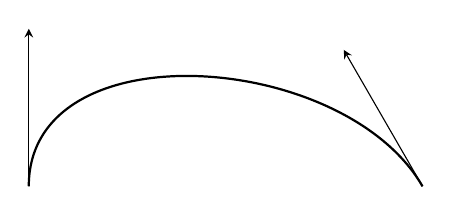
\begin{tikzpicture}
	\path(0,0) coordinate (A) (0:5) coordinate (B);
	\draw[thick](A) .. controls +(90:2) and +(120:2) .. (B);
	\draw[-stealth] (A)--++(90:2);
	\draw[-stealth] (B)--++(120:2);
\end{tikzpicture}

%------------------------------------------------------------------------------%

\section{Function Graph -- Đồ Thị Hàm Số}
Graph of function $x^3 - 3x + 1$:

\begin{tikzpicture}
	\draw[smooth] plot[domain=-2:2] (\x,{(\x)^3-3*\x+1});
\end{tikzpicture}

%------------------------------------------------------------------------------%

\section{Tangent of Curve -- Tiếp Tuyến của Đường Cong}

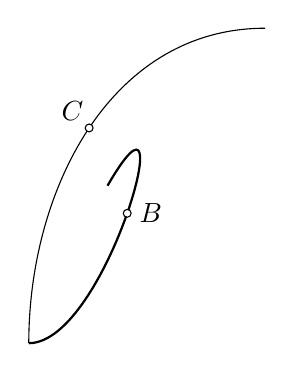
\begin{tikzpicture}
	\draw[thick] (0,0)..controls + (0:1) and +(60:2)..(1,2) coordinate[pos=.5](B);
	\draw(0,0) to[out=90,in=180] coordinate[pos=.5](C) (3,4);
	\foreach \x/\g in {B/0,C/135} \draw[fill=white] (\x) circle (.05) + (\g:.3) node{$\x$};
\end{tikzpicture}
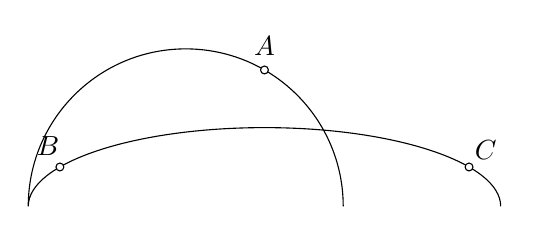
\begin{tikzpicture}
	\path
	(0,0) arc (180:60:2) coordinate (A)
	(0,0) arc (180:150:{3} and {1})  coordinate (B)
	(0,0) arc (180:30:{3} and {1})  coordinate (C)	;
	\draw
	(0,0) arc (180:0:2)
	(0,0) arc (180:0:{3} and {1});
	\foreach \x/\g in {A/90,B/120,C/45} \draw[fill=white] (\x) circle (.05) + (\g:.3) node{$\x$};
\end{tikzpicture}

\begin{tikzpicture}[line join = round,line cap=round,font=\scriptsize]
	\def\a{3}
	\def\b{1}
	\def\h{4}
	\pgfmathsetmacro\g{asin(\b/\h)}
	\pgfmathsetmacro\xo{\a *cos(\g)}
	\pgfmathsetmacro\yo{\b *sin(\g)}
	\draw[dashed]
	(\xo,\yo) arc (\g:180-\g:{\a} and {\b}) (180:\a) node[left]{$B$} --(0:\a) node[right]{$A$} (90:\h) node[above]{$S$} --(0:0) node[below left]{$O$} --(\xo,\yo) node[above right]{$M$};
	\draw (90:\h)--(-\xo,\yo) arc (180-\g:360+\g:{\a} and {\b})--cycle;
\end{tikzpicture}
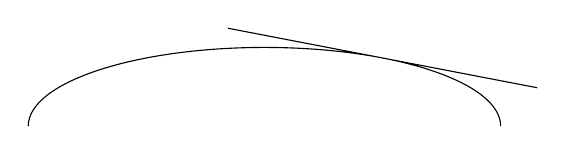
\begin{tikzpicture}
	\path
	(0:0) arc (180:60:{3} and {1}) coordinate (A)
	--([turn]0:2) coordinate (B);
	\draw (0:0) arc (180:0:{3} and {1})
	($(B)!2!(A)$)--(A)--(B);
\end{tikzpicture}

%------------------------------------------------------------------------------%

\section{Intersection of Lines -- Giao Điểm của Các Đường}

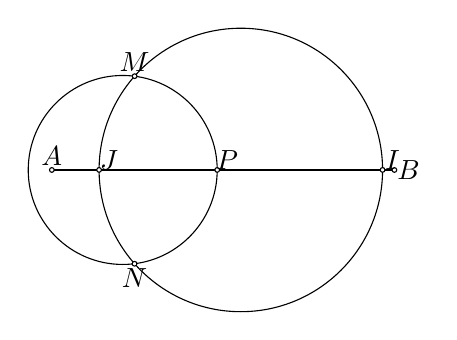
\begin{tikzpicture}[scale=.6]
	\draw[name path=ab] (-1.5,0) coordinate (A) --(5.75,0) coordinate (B);
	\draw[name path=circ1] (0,0) circle (2);
	\draw[name path=circ2] (2.5,0) circle (3);
	\path[name intersections={of=circ1 and circ2}]
	(intersection-1) coordinate (M)
	(intersection-2) coordinate (N);
	\path[name intersections={of=circ1 and ab}]
	(intersection-1) coordinate (P);
	\path[name intersections={of=circ2 and ab}]
	(intersection-1) coordinate (I)
	(intersection-2) coordinate (J);
	\foreach \x/\g in {A/90,B/0,P/45,I/45,J/45,M/90,N/-90} \draw[fill=white] (\x) circle (.05) + (\g:.3) node{$\x$};
\end{tikzpicture}
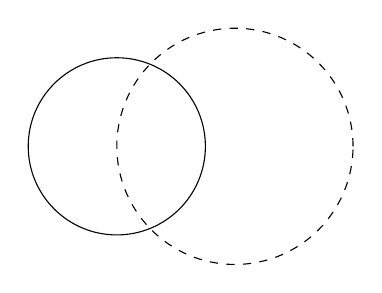
\begin{tikzpicture}[scale=.75]
	\draw (0,0) circle (1.5);
	\draw[dashed] (2,0) circle (2);
\end{tikzpicture}
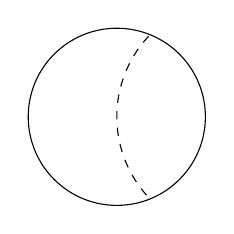
\begin{tikzpicture}[scale=.75]
	\draw (0,0) circle (1.5);
	\clip (0,0) circle (1.5);
	\draw[dashed] (2,0) circle (2);
\end{tikzpicture}
\begin{tikzpicture}
	\draw (0,0) circle (1.5);
	\begin{scope}
		\clip (0,0) circle (1.5);
		\draw[thick] (2,0) circle (2);
	\end{scope}
	\draw (1,0)--(4,0);
\end{tikzpicture}

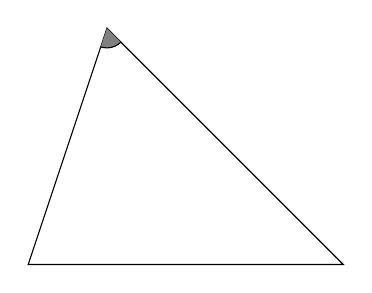
\begin{tikzpicture}
	\draw (0,0) coordinate (B) --(4,0) coordinate (C) --(1,3) coordinate (A) --cycle;
	\begin{scope}
		\clip (B)--(A)--(C);
		\draw[fill=gray] (A) circle (.25);
	\end{scope}
\end{tikzpicture}
%\begin{tikzpicture}
%	\draw (-3,0)--(3,0);
%	\path (0,0) node[above] {\includegraphics[scale=.3]{imagefile}};
%\end{tikzpicture}
\begin{tikzpicture}
	\draw (-3,0)--(3,0);
	\path (0,1.5) node{
	\begin{tikzpicture}
		\draw[fill=gray] (0,0) circle (1);
	\end{tikzpicture}};
\end{tikzpicture}

\begin{tikzpicture}
	\tikzset{dientro/.pic={\draw(-.4,-.1) rectangle (.4,.1);}}
	\draw
	(0,0) pic[local bounding box=R1] {dientro}
	(3,0) pic[local bounding box=R2] {dientro}
	(1.5,3) pic[local bounding box=R3] {dientro};
	\draw (1.75,0)--(R2)--(4,0)--(4,3)--(R3)--(-1,3)--(-1,0)--(R1)--(1.25,0);
\end{tikzpicture}
\begin{tikzpicture}
	\tikzset{dientro/.pic={\draw(-.4,-.1) rectangle (.4,.1);}}
	\draw
	(0,0) pic[local bounding box=R1] {dientro}
	(3,0) pic[local bounding box=R2] {dientro}
	(1.5,3) pic[local bounding box=R3] {dientro};
	\draw (1.75,0)--(R2)--(4,0) |-(R3) -|(-1,0) --(R1)--(1.25,0);
\end{tikzpicture}
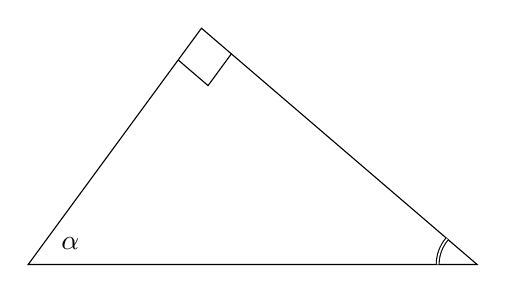
\begin{tikzpicture}
	\draw (-1.2,0) coordinate (A) --(4.5,0) coordinate (B) --(1,3) coordinate (C) --cycle;
	\draw pic[draw,double]{angle = C--B--A};
	\draw pic[draw]{right angle = B--C--A};
	\draw pic["$\alpha$",angle radius=1cm]{angle = B--A--C};
\end{tikzpicture}
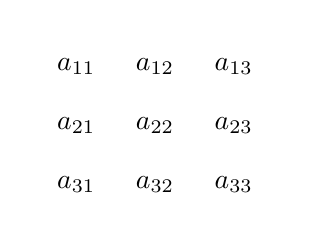
\begin{tikzpicture}
	\tikzset{bang/.style={matrix of math nodes, nodes={minimum height=.75cm,minimum width=1cm}}}
	\path
	(0,0) node[bang](A){
	a_{11}&a_{12}&a_{13}\\
	a_{21}&a_{22}&a_{23}\\
	a_{31}&a_{32}&a_{33}\\
	};
\end{tikzpicture}
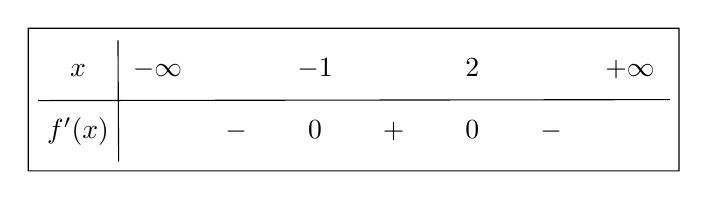
\begin{tikzpicture}
	\tikzset{bang/.style={matrix of math nodes, nodes={minimum height=.75cm,minimum width=1cm}}}
	\path
	(0,0) node[bang](A){
	x & -\infty & & -1 & & 2 & & +\infty\\
	f'(x) & & -& 0 &+ &0 &- &\\
	};
	\draw
	(A.north west) rectangle (A.south east)
	(A-1-1.south west)--(A-1-8.south east)
	(A-1-1.north east)--(A-2-1.south east)
	;
\end{tikzpicture}
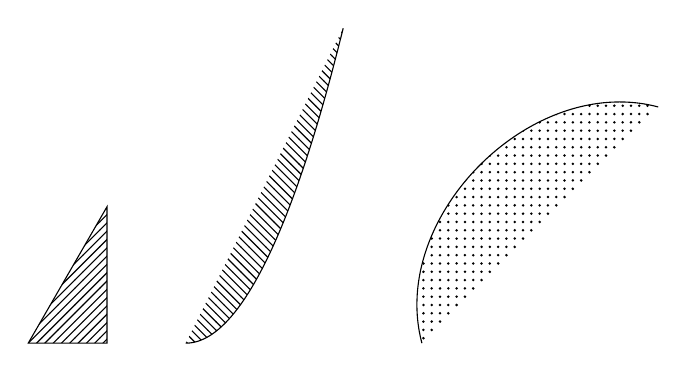
\begin{tikzpicture}
	\draw[pattern=north east lines] (0:0)--(60:2)--(0:1)--cycle;
	\draw[pattern=north west lines] (2,0) parabola (4,4);
	\draw[pattern=dots] (5,0) to[bend left=60] (8,3);
\end{tikzpicture}

%------------------------------------------------------------------------------%

\section{Shading}


\begin{tikzpicture}
	\fill[ball color=red] (0,0) circle (1);
	\shade[top color=blue,bottom color=orange,middle color=white] (2,-1) rectangle (6,1);
\end{tikzpicture}
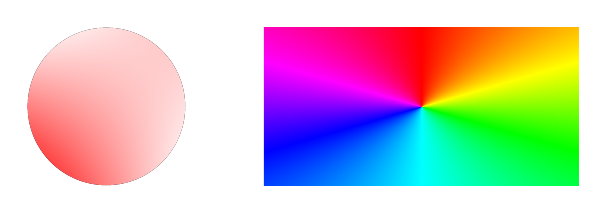
\begin{tikzpicture}
	\fill[lower left=red,upper right=pink] (0,0) circle (1);
	\shade[shading=color wheel] (2,-1) rectangle (6,1);
\end{tikzpicture}


\begin{tikzpicture}
	\fill[outer color=blue] (0,0) circle (1);
	\shade[inner color=yellow] (2,-1) rectangle (6,1);
\end{tikzpicture}

\begin{tikzpicture}
	\foreach \i in {1,...,20}\draw(0,.1*\i)--++(0:2);
\end{tikzpicture}
\begin{tikzpicture}
	\foreach \i in {1,...,3}{
		\foreach \j in {1,...,4}
			\path(\i,\j) node{$a_{\i \j}$};
	}
\end{tikzpicture}
\begin{tikzpicture}
	\foreach \i in {1,...,3}{
		\foreach \j in {1,...,4}
		\pgfmathsetmacro{\ht}{int(\i+\j)}
			\path(\i,\j) node{\ht};
	}
\end{tikzpicture}

\begin{tikzpicture}
	\foreach \x/\col in {1/red, 2/blue, 3/orange, 4/pink, 5/yellow, 6/gray}
	\fill[\col] (\x,0) rectangle +(.5,2);
\end{tikzpicture}
\begin{tikzpicture}
	\foreach \col[count=\x from 1] in {red, blue, orange, pink, yellow, gray}
	\fill[\col] (\x,0) rectangle +(.5,2);
\end{tikzpicture}
\begin{tikzpicture}
	\def\chamtron(#1,#2)(#3){
	\fill[gray](#1,#2) circle (#3);
	}
	\chamtron(0,0)(.2)
	\chamtron(1,0)(.3)
	\chamtron(0,2)(.5)
\end{tikzpicture}

%\begin{tikzpicture}[join=round,cap=round]
%	\def\chanphangiac(#1,#2,#3)(#4){
%	\path
%	($(#2)!1mm!(#1)$) coordinate (#2#1)
%	($(#2)!1mm!(#3)$) coordinate (#2#3)
%	($(#2#1)!.5(#2#3)$) coordinate (#2t)
%	(intersection of #2--#2t and #1--#3) coordinate (#4)
%	;
%	}
%	\path
%	(1,3) coordinate (A)
%	(0,0) coordinate (B)
%	(5,0) coordinate (C)
%	;
%	\chanphangiac(B,A,C)(D)
%	\chanphangiac(A,B,C)(E)
%	\chanphangiac(B,C,A)(F)
%	\draw (A)--(B)--(C)--cycle (A)--(D) (B)--(E) (C)--(F);
%	\foreach \x/\g in {A/90,B/180,C/0,D/-90,E/0,F/180}
%	\draw[fill=white] (\x) circle (.05) + (\g:.3) node{$\x$};
%\end{tikzpicture}

\begin{tikzpicture}
	\def\r{2}
	\path
	(0:0) coordinate (I)
	(I)+(130:\r) coordinate (A)
	(I)+(180:\r) coordinate (B)
	(I)+(0:\r) coordinate (C)
	;
	\draw
	(I) circle (\r)
	(A)--(B)--(C)--cycle;
	\foreach \x/\g in{A/90,B/180,C/0,I/-90} \draw[fill=white] (\x) circle (.05) + (\g:.3) node{$\x$};
\end{tikzpicture}
\begin{tikzpicture}
	\def\r{3}\def\d{9}\def\gM{-150}
	\path
	(0:0) coordinate (O)
	(180:\d) coordinate (C)
	(\gM:\r) coordinate (M)
	($(O)!.5!(C)$) coordinate (Ot)
	($(C)!(O)!(M)$) coordinate (I)
	($(M)!2!(I)$) coordinate (N)
	($(M)!1mm!90:(O)$) coordinate (Mt)
	;
	\path[name path = c1] (O) circle (\r);
	\path[name path = c2] (Ot) let \p1=($(O)-(Ot)$) in circle ({veclen(\x1,\y1)});
	\path[name intersections = {of = c1 and c2, by = {A,B}}]
	(intersection of A--B and O--C) coordinate (H)
	(intersection of A--B and M--N) coordinate (K)
	(intersection of M--Mt and C--A) coordinate (E)
	(intersection of M--Mt and C--B) coordinate (F)
	($(O)+(A)-(H)$) coordinate (Op)
	(intersection of O--Op and C--A) coordinate (P)
	(intersection of O--Op and C--B) coordinate (Q)
	;
	\pgfresetboundingbox
	\draw
	(O) circle (\r)
	(C)--(A)--(O) --(B)--cycle
	(O)--(C)--(N) (A)--(B) (M)--(O)--(I) (E)--(F) (N)--(A)--(M) (A)--(P)--(Q)--(B)
	;
	\foreach \x/\y/\z in {O/I/N,A/H/O,O/M/E,O/A/P,O/B/Q} \pic[draw, angle radius=2mm]{right angle=\x--\y--\z};
	\foreach \x/\g in {O/-30,C/180,A/120,B/-150,E/120,F/-120,M/-150,Q/-90,P/90,H/120,K/-135,N/-45,I/-90} \draw[fill=white] (\x) circle (.05) + (\g:.3) node{$\x$};
\end{tikzpicture}

\section{Triangle}

\begin{tikzpicture}
	\def\r{1.5}
	\path
	(130:\r) coordinate (A)
	(180:\r) coordinate (B)
	(0:\r) coordinate (C)
	;
	\draw
	(A)--(B)--(C)--cycle
	pic[draw, angle radius=2mm]{right angle=B--A--C}
	;
	\foreach \x/\g in {A/90,B/180,C/0} \draw[fill=white] (\x) circle (.05) + (\g:.3) node{$\x$};
\end{tikzpicture}
\begin{tikzpicture}
	\path
	(0:0) coordinate (A)
	(0:3) coordinate (B)
	($(A)!2cm!90:(B)$) coordinate (C)
	;
	\draw
	(A)--(B)--(C)--cycle
	pic[draw, angle radius=2mm]{right angle=B--A--C}
	;
	\foreach \x/\g in {A/-135,B/0,C/90} \draw[fill=white] (\x) circle (.05) + (\g:.3) node{$\x$};
\end{tikzpicture}

%------------------------------------------------------------------------------%

\section{Miscellaneous}

%------------------------------------------------------------------------------%

\printbibliography[heading=bibintoc]
	
\end{document}